Achieving practical exascale supercomputing will require massive increases in energy efficiency.  
The bulk of this improvement will likely be derived from hardware advances such as improved semiconductor device technologies and tighter integration, hopefully resulting in more energy efficient computer architectures.  
Still, software will have an important role to play.  
With every generation of new hardware, more power measurement and control capabilities are exposed. 
Many of these features require software involvement to maximize feature benefits.
This trend will allow algorithm designers to add power and energy efficiency to their optimization criteria.  
Similarly, at the system level, opportunities now exist for energy-aware scheduling to meet external utility constraints such as time of day cost charging and power ramp rate limitations.  
Finally, future architectures might not be able to operate all components at full capability for a range of reasons including temperature considerations or power delivery limitations.
Software will need to make appropriate choices about how to allocate the available power budget given many, sometimes conflicting considerations.

For these reasons, we have developed a portable API for power measurement and control.  
This Power API provides multiple levels of abstractions to satisfy the requirements of multiple types of users~\cite{Laros:2013:PwrUseCase}.
The remainder of this document describes the details of this Power API specification.


\section{Background}\label{sec:Background}
We draw our inspiration from efforts such as the MPI forum's\footnote{http://www.mpi-forum.org} process. 
We seek to develop a de facto standard, led by a neutral national laboratory, which is funded by a neutral federal agency.
Community involvement is critical to the effort.
The laboratory team has been garnering participation by making presentations at workshops and operational group meetings. 
We desire community participation from university and other researchers, as well as HPC practitioners. 
Concurrent with the specification development, the authors are creating a reference implementation comprising a subset of the overall API functionality. 
This task is important to ensure that the specification is usable. 
The ultimate goal, however, is that vendors of the hardware and software components provide their own implementations. 
It is likely that some portion of these functions have already been written by vendors, but with slightly different calling arguments.
For portability sake, we are hopeful that the specific implementations can be melded to this proposed community API.

\section{Motivation}\label{sec:Motivation}
The introductory paragraph above, offers a few examples where a Power API would be useful. 
This document's abstract provides references to a small subset of the current research activities that would benefit from a community-adopted power API.
Additional, more fleshed out examples are described in the appendices of the \emph{Power/Energy Use Cases for High Performance Computing} document~\cite{Laros:2013:PwrUseCase}.
To provide the proper mindset for reading this document, we offer the following list as well.
\begin{itemize}
\item A job is entering a checkpoint phase. The application requests a reduced processor frequency during the long I/O period.
\item A developer is trying to understand frequency sensitivity of an algorithm and starts a tool that analyzes performance and power consumption while the job is running.
\item Once an application's power signature is analyzed, future job submissions give power hints to the resource manager.
\item A data center has a maximum of capacity of nn MW. One HPC system is down for extended maintenance. Other systems can have a higher maximum power cap.
\item For electric bills based on peak usage periods, determine a maximum HPC load that minimizes loss of HPC use. Then direct the scheduler to enforce that peak usage.
\end{itemize}

\section{Use Case Development}\label{sec:UseCase}
The \emph{Power/Energy Use Cases for High Performance Computing} document~\cite{Laros:2013:PwrUseCase} identifies the requirements for the Power API.
Rather than a list, the requirements are specified as formal use cases employing the ISO/IEC 19501:2005 Unified Modeling Language (UML) standard, which is described in the reference manual by Booch, et al.~\cite{GangOfThree:1999}.
While the term use case has come to be almost synonymous with scenario, the standard defines a use case \emph{model}.
The use case model does include scenario-like requirement specifications, but it also clearly identifies the roles and scope of the requirements. 
For this document, the key concepts from the use case model are \emph{actor} and \emph{system}.
Each identified actor plays a distinct role in using the power API. 
Actors can be persons, other systems, or something else (e.g. cron, asynchronous event, etc.). 
For the Power API use case model, an HPC computer is broken down into logical systems.
By breaking down the requirements into this use case model, we can clearly see the demarcation points requiring an API between external actors and each system. 
And by subsequently viewing systems as actors to the other systems, we obtain the complete set of necessary interfaces.
 
\begin{figure}[!ht]
    \begin{center}
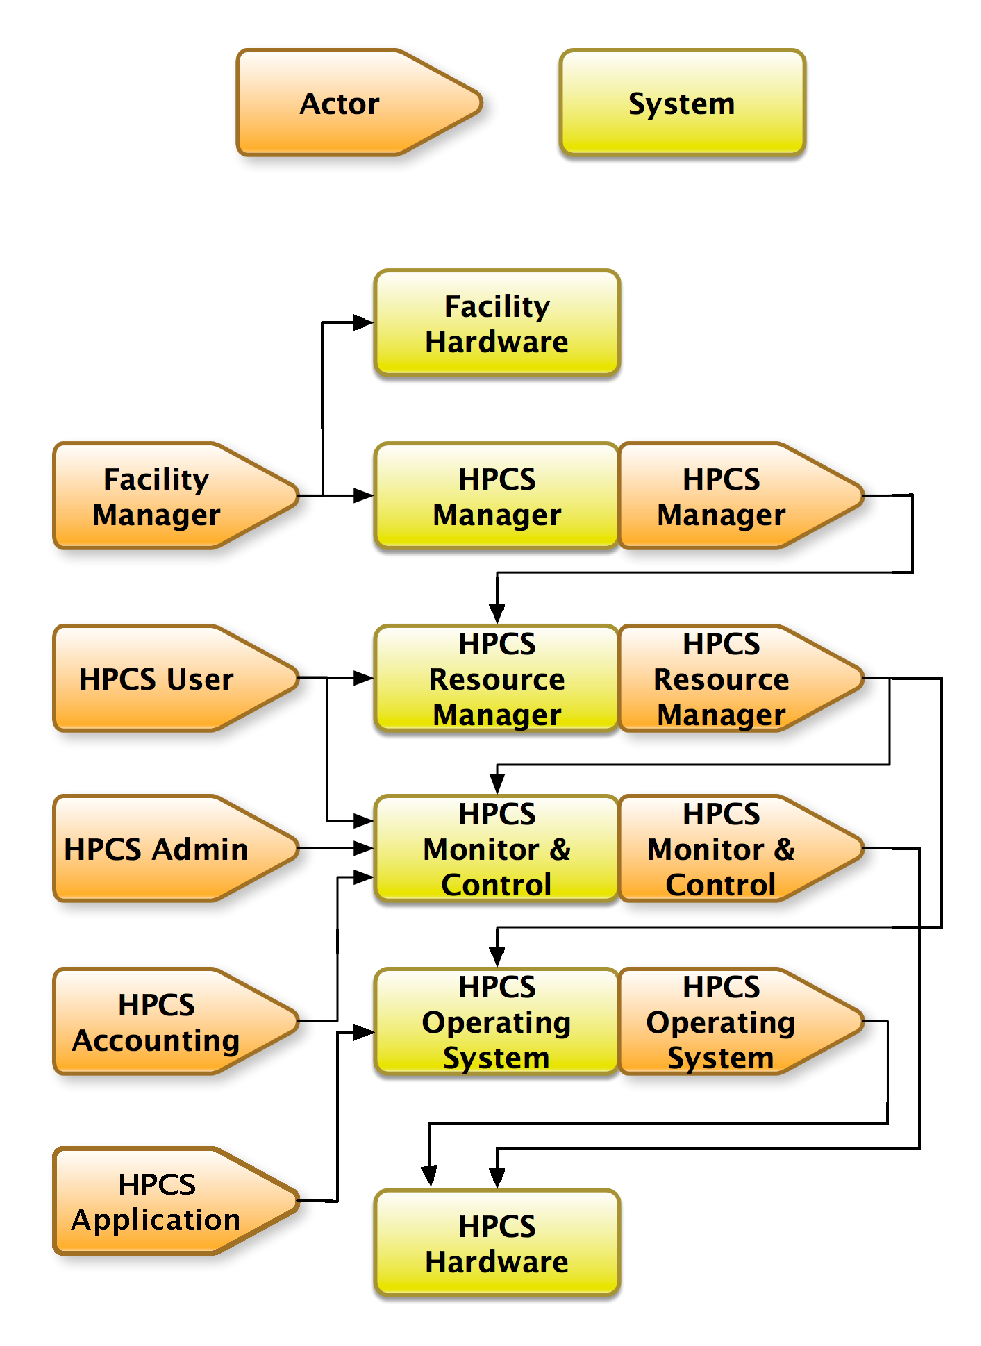
\includegraphics[height=0.6\textheight,width=.69\linewidth]{FIGURES/TopLevelDiagram}
    \end{center}
\caption{Top Level Conceptual Diagram representing the culmination of all Use Case Diagrams covered.}
\label{fig:UCDTopLevel}
\end{figure}

The specific actor/system pairs used for the power API are shown in Figure \ref{fig:UCDTopLevel}.
The external actors are shown on the left portion of the diagram. 
Systems are shown as rectangles. 
The four systems conjoined with the actor symbol also serve as actors for some use cases. 
The ten sections within Chapter \ref{chap:Interfaces} provide function specifications for the ten actor/system pairs (Role/System pairs in the specification).
The two missing interfaces are Facility Manager to Facility Hardware and Facility Manager to HPCS manager.
These were included in the use case model to identify the boundaries of the specification and recognize important points of information input. 

\section{Security Model}\label{sec:SecModel}
The specification assumes traditional hardware (e.g. protection rings) and operating system support for access control.
Implementations should only need traditional restrictions based on authenticated individual identity and/or the groups to which the individual belongs.
A super user is likely needed as well.
Depending on the implementation, the context structure (Section \ref{sec:ContextTypeDefinitions}) may be sufficiently protected to allow for secure storage of access information. Future releases of the specification will address security and policy considerations in more detail.
